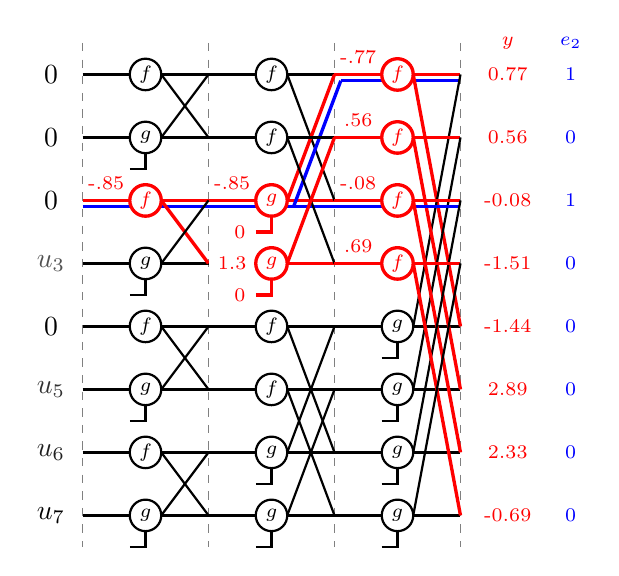
\begin{tikzpicture}[scale=.8, thick]

  \draw[very thin,gray,dashed] (1,.5) -- (1,-7.5);
  \draw[very thin,gray,dashed] (3,.5) -- (3,-7.5);
  \draw[very thin,gray,dashed] (5,.5) -- (5,-7.5);
  \draw[very thin,gray,dashed] (7,.5) -- (7,-7.5);

  %\node at (-.5,1) {layer};
  %\node at (1,1) {0};
  %\node at (3,1) {1};
  %\node at (5,1) {2};
  %\node at (7,1) {3};

  \node at (.5,0) {\color{black}$0$};
  \node at (.5,-1) {\color{black}$0$};
  \node at (.5,-2) {\color{black}$0$};
  \node at (.5,-3) {\color{black!68.4}$u_3$};
  \node at (.5,-4) {\color{black}$0$};
  \node at (.5,-5) {\color{black!80.9}$u_5$};
  \node at (.5,-6) {\color{black!87.9}$u_6$};
  \node at (.5,-7) {\color{black!99.6}$u_7$};

  \draw (1,0) -- ++(.75,0);
  \draw (2.25,0) -- ++(.75,0);
  \draw (1,-1) -- ++(.75,0);
  \draw (2.25,-1) -- ++(.75,0);

  \draw (2,0) circle [radius=.25] node {\scriptsize $f$};
  \draw (2,-1) circle [radius=.25] node {\scriptsize $g$};
  
  \draw (3,-1) -- ++(-.75,1);
  \draw (3,0) -- ++(-.75,-1);
  
  \draw (1.75,-1.5) -- ++(.25,0) -- ++(0,.25);

  \draw[red,very thick] (1,-2) -- ++(.75,0) node [above,midway] {\scriptsize-$.85$};
  \draw[blue,very thick] (1,-2.1) -- ++(.75,0);
  \draw[red,very thick] (2.25,-2) -- ++(.75,0);
  \draw[blue,very thick] (2.25,-2.1) -- ++(.75,0);
  \draw (1,-3) -- ++(.75,0);
  \draw (2.25,-3) -- ++(.75,0);

  \draw[red,very thick] (2,-2) circle [radius=.25] node {\scriptsize $f$};
  \draw (2,-3) circle [radius=.25] node {\scriptsize $g$};
  
  \draw[red,very thick] (3,-3) -- ++(-.75,1);
  \draw (3,-2) -- ++(-.75,-1);
  
  \draw (1.75,-3.5) -- ++(.25,0) -- ++(0,.25);

  \draw (1,-4) -- ++(.75,0);
  \draw (2.25,-4) -- ++(.75,0);
  \draw (1,-5) -- ++(.75,0);
  \draw (2.25,-5) -- ++(.75,0);

  \draw (2,-4) circle [radius=.25] node {\scriptsize $f$};
  \draw (2,-5) circle [radius=.25] node {\scriptsize $g$};
  
  \draw (3,-5) -- ++(-.75,1);
  \draw (3,-4) -- ++(-.75,-1);
  
  \draw (1.75,-5.5) -- ++(.25,0) -- ++(0,.25);

  \draw (1,-6) -- ++(.75,0);
  \draw (2.25,-6) -- ++(.75,0);
  \draw (1,-7) -- ++(.75,0);
  \draw (2.25,-7) -- ++(.75,0);

  \draw (2,-6) circle [radius=.25] node {\scriptsize $f$};
  \draw (2,-7) circle [radius=.25] node {\scriptsize $g$};
  
  \draw (3,-7) -- ++(-.75,1);
  \draw (3,-6) -- ++(-.75,-1);
  
  \draw (1.75,-7.5) -- ++(.25,0) -- ++(0,.25);

%-----

  \draw (3,0) -- ++(.75,0);
  \draw (4.25,0) -- ++(.75,0);
  \draw[red,very thick] (3,-2) -- ++(.75,0) node [above,midway] {\scriptsize-$.85$};
  \draw[blue,very thick] (3,-2.1) -- ++(.75,0);
  \draw[red,very thick] (4.25,-2) -- ++(.75,0);
  \draw[blue,very thick] (4.25,-2.1) -- ++(.75,0);

  \draw (4,0) circle [radius=.25] node {\scriptsize $f$};
  \draw[red,very thick] (4,-2) circle [radius=.25] node {\scriptsize $g$};
  
  \draw (5,-2) -- ++(-.75,2);
  \draw[red,very thick] (5,0) -- ++(-.75,-2);
  \draw[blue,very thick] (5.1,-.1) -- ++(-.75,-2);
  
  \draw[red,very thick] (3.75,-2.5) -- ++(.25,0) -- ++(0,.25);
  \node[red] at (3.5,-2.5) {\scriptsize$0$};

  \draw (3,-1) -- ++(.75,0);
  \draw (4.25,-1) -- ++(.75,0);
  \draw[red,very thick] (3,-3) -- ++(.75,0) node [midway,fill=white] {\scriptsize$1.3$};
  \draw[red,very thick] (4.25,-3) -- ++(.75,0);

  \draw (4,-1) circle [radius=.25] node {\scriptsize $f$};
  \draw[red,very thick] (4,-3) circle [radius=.25] node {\scriptsize $g$};
  
  \draw (5,-3) -- ++(-.75,2);
  \draw[red,very thick] (5,-1) -- ++(-.75,-2);
  
  \draw[red,very thick] (3.75,-3.5) -- ++(.25,0) -- ++(0,.25);
  \node[red] at (3.5,-3.5) {\scriptsize$0$};

  \draw (3,-4) -- ++(.75,0);
  \draw (4.25,-4) -- ++(.75,0);
  \draw (3,-6) -- ++(.75,0);
  \draw (4.25,-6) -- ++(.75,0);

  \draw (4,-4) circle [radius=.25] node {\scriptsize $f$};
  \draw (4,-6) circle [radius=.25] node {\scriptsize $g$};
  
  \draw (5,-6) -- ++(-.75,2);
  \draw (5,-4) -- ++(-.75,-2);
  
  \draw (3.75,-6.5) -- ++(.25,0) -- ++(0,.25);

  \draw (3,-5) -- ++(.75,0);
  \draw (4.25,-5) -- ++(.75,0);
  \draw (3,-7) -- ++(.75,0);
  \draw (4.25,-7) -- ++(.75,0);

  \draw (4,-5) circle [radius=.25] node {\scriptsize $f$};
  \draw (4,-7) circle [radius=.25] node {\scriptsize $g$};
  
  \draw (5,-7) -- ++(-.75,2);
  \draw (5,-5) -- ++(-.75,-2);
  
  \draw (3.75,-7.5) -- ++(.25,0) -- ++(0,.25);

%-----

  \draw[red,very thick] (5,0) -- ++(.75,0) node [above,midway] {\scriptsize-$.77$};
  \draw[blue,very thick] (5.1,-.1) -- ++(.65,0);
  \draw[red,very thick] (6.25,0) -- ++(.75,0);
  \draw[blue,very thick] (6.25,-.1) -- ++(.75,0);
  \draw (5,-4) -- ++(.75,0);
  \draw (6.25,-4) -- ++(.75,0);

  \draw[red,very thick] (6,0) circle [radius=.25] node {\scriptsize $f$};
  \draw (6,-4) circle [radius=.25] node {\scriptsize $g$};
  
  \draw[red,very thick] (7,-4) -- ++(-.75,4);
  \draw (7,0) -- ++(-.75,-4);
  
  \draw (5.75,-4.5) -- ++(.25,0) -- ++(0,.25);

  \draw[red,very thick] (5,-1) -- ++(.75,0) node [above,midway] {\scriptsize$.56$};
  \draw[red,very thick] (6.25,-1) -- ++(.75,0);
  \draw (5,-5) -- ++(.75,0);
  \draw (6.25,-5) -- ++(.75,0);

  \draw[red,very thick] (6,-1) circle [radius=.25] node {\scriptsize $f$};
  \draw (6,-5) circle [radius=.25] node {\scriptsize $g$};
  
  \draw[red,very thick] (7,-5) -- ++(-.75,4);
  \draw (7,-1) -- ++(-.75,-4);
  
  \draw (5.75,-5.5) -- ++(.25,0) -- ++(0,.25);

  \draw[red,very thick] (5,-2) -- ++(.75,0) node [above,midway] {\scriptsize-$.08$};
  \draw[blue,very thick] (5,-2.1) -- ++(.75,0);
  \draw[red,very thick] (6.25,-2) -- ++(.75,0);
  \draw[blue,very thick] (6.25,-2.1) -- ++(.75,0);
  \draw (5,-6) -- ++(.75,0);
  \draw (6.25,-6) -- ++(.75,0);

  \draw[red,very thick] (6,-2) circle [radius=.25] node {\scriptsize $f$};
  \draw (6,-6) circle [radius=.25] node {\scriptsize $g$};
  
  \draw[red,very thick] (7,-6) -- ++(-.75,4);
  \draw (7,-2) -- ++(-.75,-4);
  
  \draw (5.75,-6.5) -- ++(.25,0) -- ++(0,.25);

  \draw[red,very thick] (5,-3) -- ++(.75,0) node [above,midway] {\scriptsize$.69$};
  \draw[red,very thick] (6.25,-3) -- ++(.75,0);
  \draw (5,-7) -- ++(.75,0);
  \draw (6.25,-7) -- ++(.75,0);

  \draw[red,very thick] (6,-3) circle [radius=.25] node {\scriptsize $f$};
  \draw (6,-7) circle [radius=.25] node {\scriptsize $g$};
  
  \draw[red,very thick] (7,-7) -- ++(-.75,4);
  \draw (7,-3) -- ++(-.75,-4);
  
  \draw (5.75,-7.5) -- ++(.25,0) -- ++(0,.25);
  
  \node at (7.75,.5) {\scriptsize\color{red}$\bm{y}$};
  \node at (7.75,0) {\scriptsize\color{red}$0.77$};
  \node at (7.75,-1) {\scriptsize\color{red}$0.56$};
  \node at (7.75,-2) {\scriptsize\color{red}-$0.08$};
  \node at (7.75,-3) {\scriptsize\color{red}-$1.51$};
  \node at (7.75,-4) {\scriptsize\color{red}-$1.44$};
  \node at (7.75,-5) {\scriptsize\color{red}$2.89$};
  \node at (7.75,-6) {\scriptsize\color{red}$2.33$};
  \node at (7.75,-7) {\scriptsize\color{red}-$0.69$};
  
  \node at (8.75,.5) {\scriptsize\color{blue}$\bm{e}_2$};
  \node at (8.75,0) {\scriptsize\color{blue}$1$};
  \node at (8.75,-1) {\scriptsize\color{blue}$0$};
  \node at (8.75,-2) {\scriptsize\color{blue}$1$};
  \node at (8.75,-3) {\scriptsize\color{blue}$0$};
  \node at (8.75,-4) {\scriptsize\color{blue}$0$};
  \node at (8.75,-5) {\scriptsize\color{blue}$0$};
  \node at (8.75,-6) {\scriptsize\color{blue}$0$};
  \node at (8.75,-7) {\scriptsize\color{blue}$0$};

\end{tikzpicture}